\chapter{Proofs}

\section{Measures on parallelogram grid dispersion} \label{sec:proof_pargrid_measures}
The parallelogram dispersion of points on object surfaces occurs when sample points which are arranged in a square grid on the image plane are projected onto the object surface. The rays are perpendicular to the image plane, as a parallel projection camera is supposed for the point cloud.  

This is shown on the figure \ref{fig:lattice_proof}. Here the image space spans the XY plane. $16$ pixels from the image space (in blue) are shown as the intersections of the square grid. $PO$ is the origin point with coordinates $(0, 0)$, and $PX = (p_l, 0)$, $PY = (0, p_l)$ are the first points in X and Y direction. Their equivalents on the object surface (in light gray) are $O, X, Y$. $\vec{n}$ is the normal vector of this surface. The parallelogram grid on it is the projection of the square grid from the image space.

The points on the object surface form a lattice, for which the grid represents one possible basis. Others would be possible, for example one where the parallelograms have an edge joining $X$ and $Y$. In general, a lattice can be defined as the set of points in $\mathbb{R}^2$
\begin{equation}
\left\{ a \vec{v} + b \vec{u} : a,b \in \mathbb{Z} \right\}
\end{equation}
Where $\vec{v}, \vec{u} \in \mathbb{R}^2$ are two vectors forming one of infinitely possible bases for this lattice. On this example $\vec{v} = OX$ and $\vec{u} = OY$ is one basis.

$l_\text{min}$ is defined to be the shortest possible Euclidian distance between any two of these lattice points. On the image space, $d(PO, PX) = d(PO, PY) = p_l$ is the shortest distance, whereas $d(PX, PY) = p_l \, \sqrt{2} > p_l$. The example on the figure is set so that $d(X, Y) < d(O, X) < d(O, Y)$, and $d(X, Y)$ is the shortest distance. By making the surface even more oblique, it is also possible that two points that are even more far off in image space become the closest points on the projection. In general, the problem of finding $l_\text{min}$ on a lattice is known as the \emph{shortest vector problem}. For this two-dimensional case, a simple algorithm exists for finding the minimal basis consisting of the shortest and second-shortest vector. \cite{Galb2012}

Because the lattice is invariant to a translation of the object surface plane $P$ in space, let $P$ pass through the origin. For any vector $\vec{p} = \transpose{(p_x, p_y)}$ on the image plane, the three-dimensional coordinates of the projected vector on the object surfaces become
\begin{equation}
\vec{p'} = \transpose{\left( p_x, p_y, - \frac{n_x \, p_x + n_y \, p_y}{n_z}  \right)}
\end{equation}
Its norm is
\begin{equation}
\| \vec{p'} \| = \sqrt{p^2_x + p^2_y + \frac{(n_x p_x + n_y p_y)^2}{n^2_z}}
\end{equation}
The square grid points on image space have the coordinates
\begin{equation}
\left\{ (x \, p_l, y \, p_l) : x,y \in \mathbb{Z} \right\}
\end{equation}

For any segment joining two points on the grid, an identical segment exists where the first point is the origin $O$. So to find the shortest segment it is sufficient to compare the lengths $\| \vec{p'} \|$ where $\vec{p}$ is the vector from the origin to another point on the image space lattice. So the shortest length would be the result of
\begin{equation}
l_{\text{min}} = p_l \, \min_{\substack{x,y \in \mathbb{Z} \\ (x,y) \neq (0,0)}} d(x,y)
\hspace{4mm} \text{where} \hspace{4mm}
d(x,y) = \| \vec{p'} \|
\hspace{4mm} \text{and} \hspace{4mm}
\vec{p} = \transpose{(x, y)}
\end{equation}
This function $d$ has the property that $d(-x,-y) = d(x,y)$, and so it is sufficient to only test the values where $y \geq 0$.

\subsection{Approximation}
In most cases, when the surface is not too oblique, the minimum for $(x, y)$ is found in $\{ (0, 1), (0, 1), (1, 1), (-1, 1) \}$. This can be seen be visualizing the function $d(x,y)$ for a given $\vec{n}$. Figure \ref{fig:lmin_d_func} shows some examples. The color gradient shows the value of the function on a logarithmic scale, where blue represents the lowest values. The goal is to find the points where $x$ and $y$ are integers for which the function is minimal.

By taking the minimum of $\| \vec{p'} \|$ for those four values of $(x, y)$, the formula in \ref{eq:pargrid_lmin} is obtained.

\begin{figure}[h]
\begin{subfigure}{.49\textwidth}
	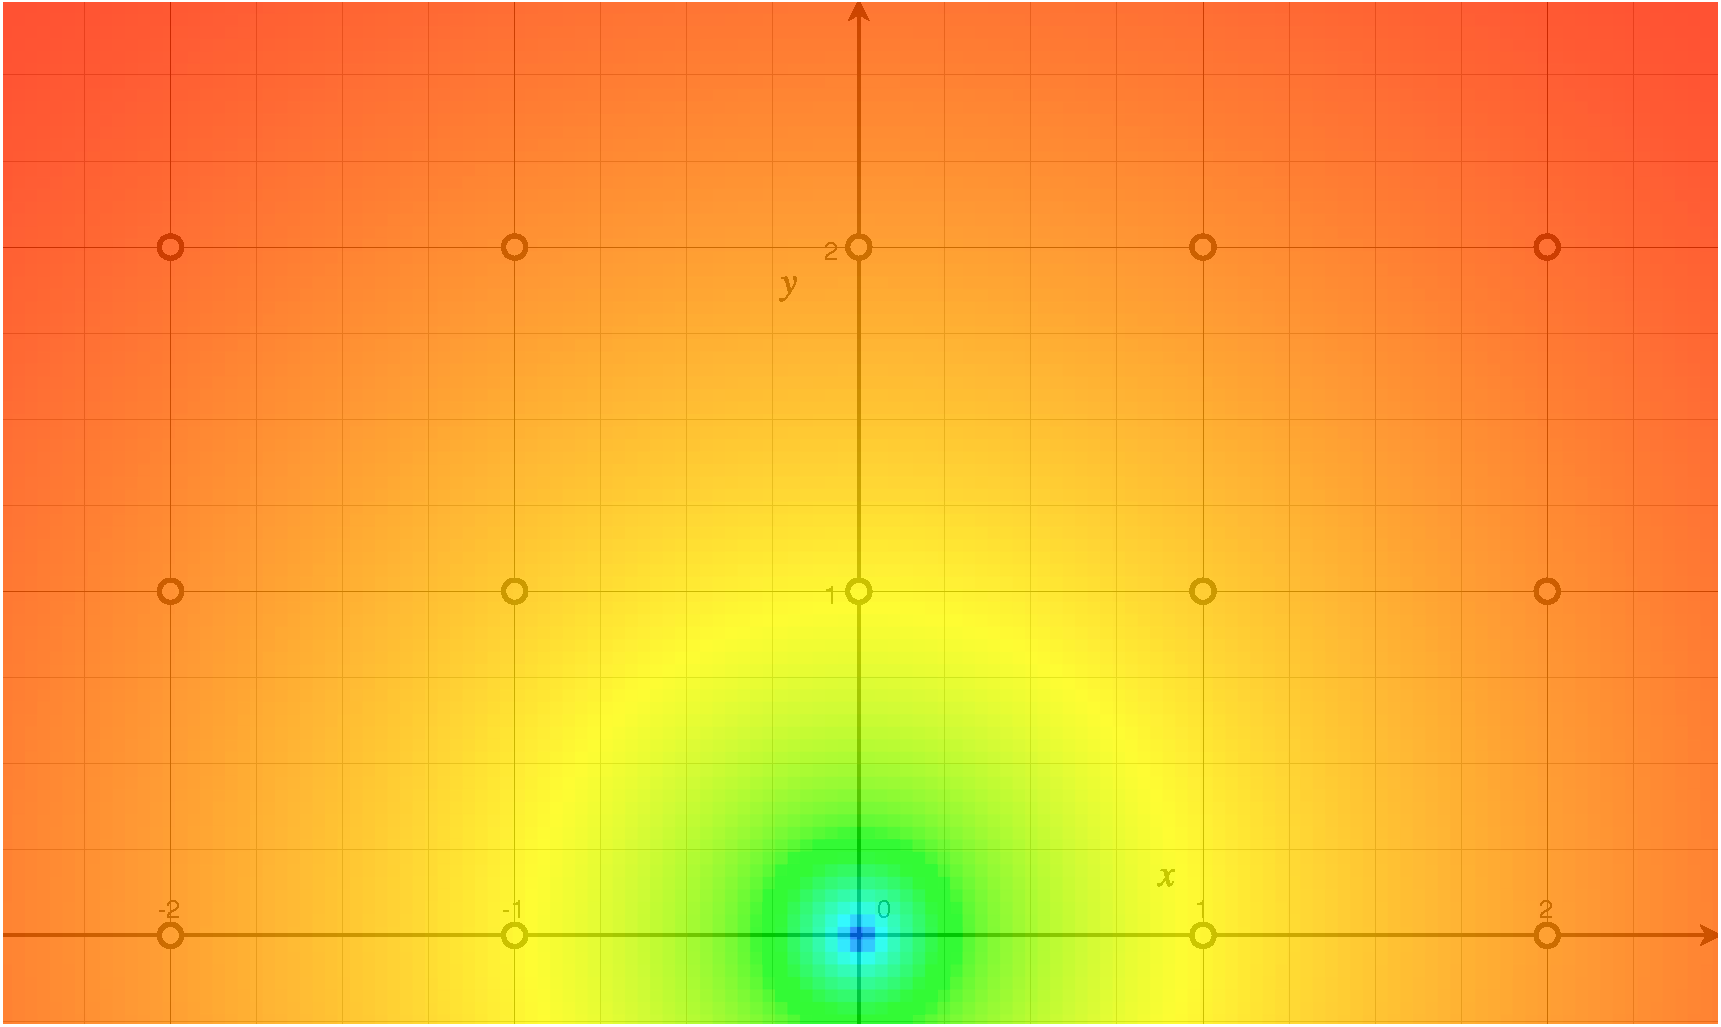
\includegraphics[width=\linewidth]{fig/lmin/0-0-1.pdf}
	\caption{$\vec{n} = \transpose{(0, 0, 1)}$. min: $(0, 1)$ or $(1, 0)$}
\end{subfigure}%
\begin{subfigure}{.49\textwidth}
	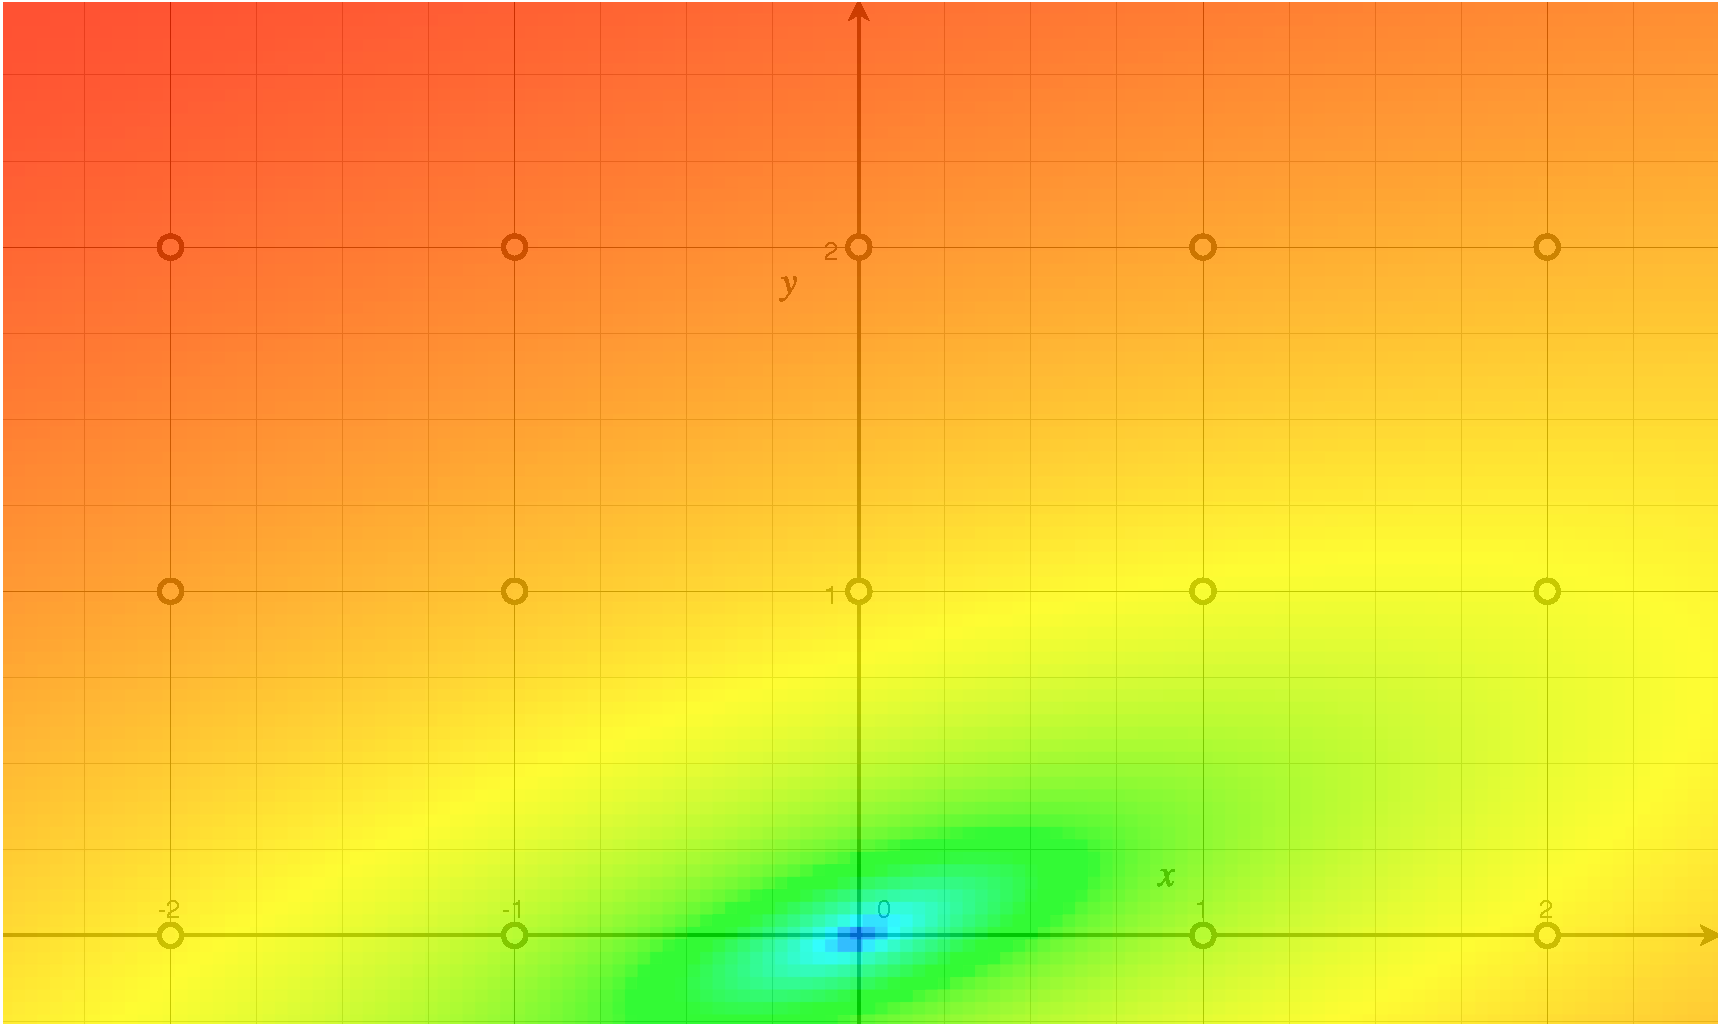
\includegraphics[width=\linewidth]{fig/lmin/1--3-1.pdf}
	\caption{$\vec{n} = \transpose{(0.302, -0.905, 0.302)}$. min: $(0, 1)$}
\end{subfigure}\\
\begin{subfigure}{.49\textwidth}
	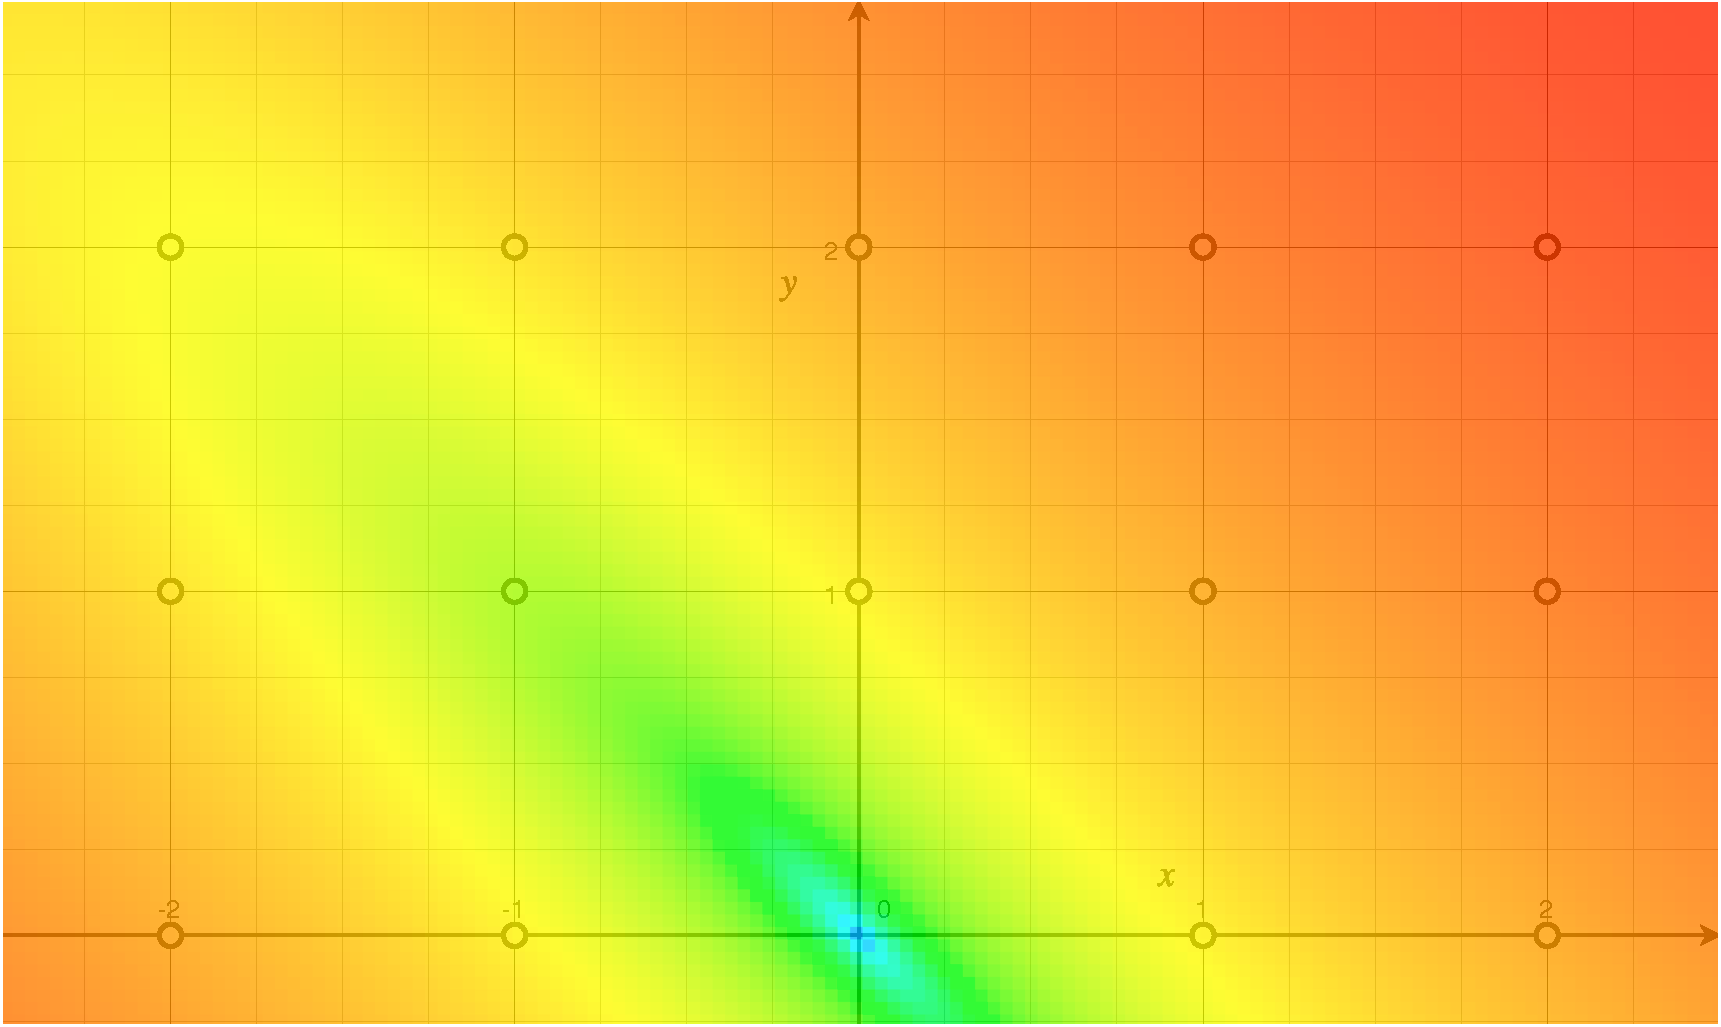
\includegraphics[width=\linewidth]{fig/lmin/3-3-1.pdf}
	\caption{$\vec{n} = \transpose{(0.688, 0.688, 0.299)}$. min: $(-1, 1)$}
\end{subfigure}%
\begin{subfigure}{.49\textwidth}
	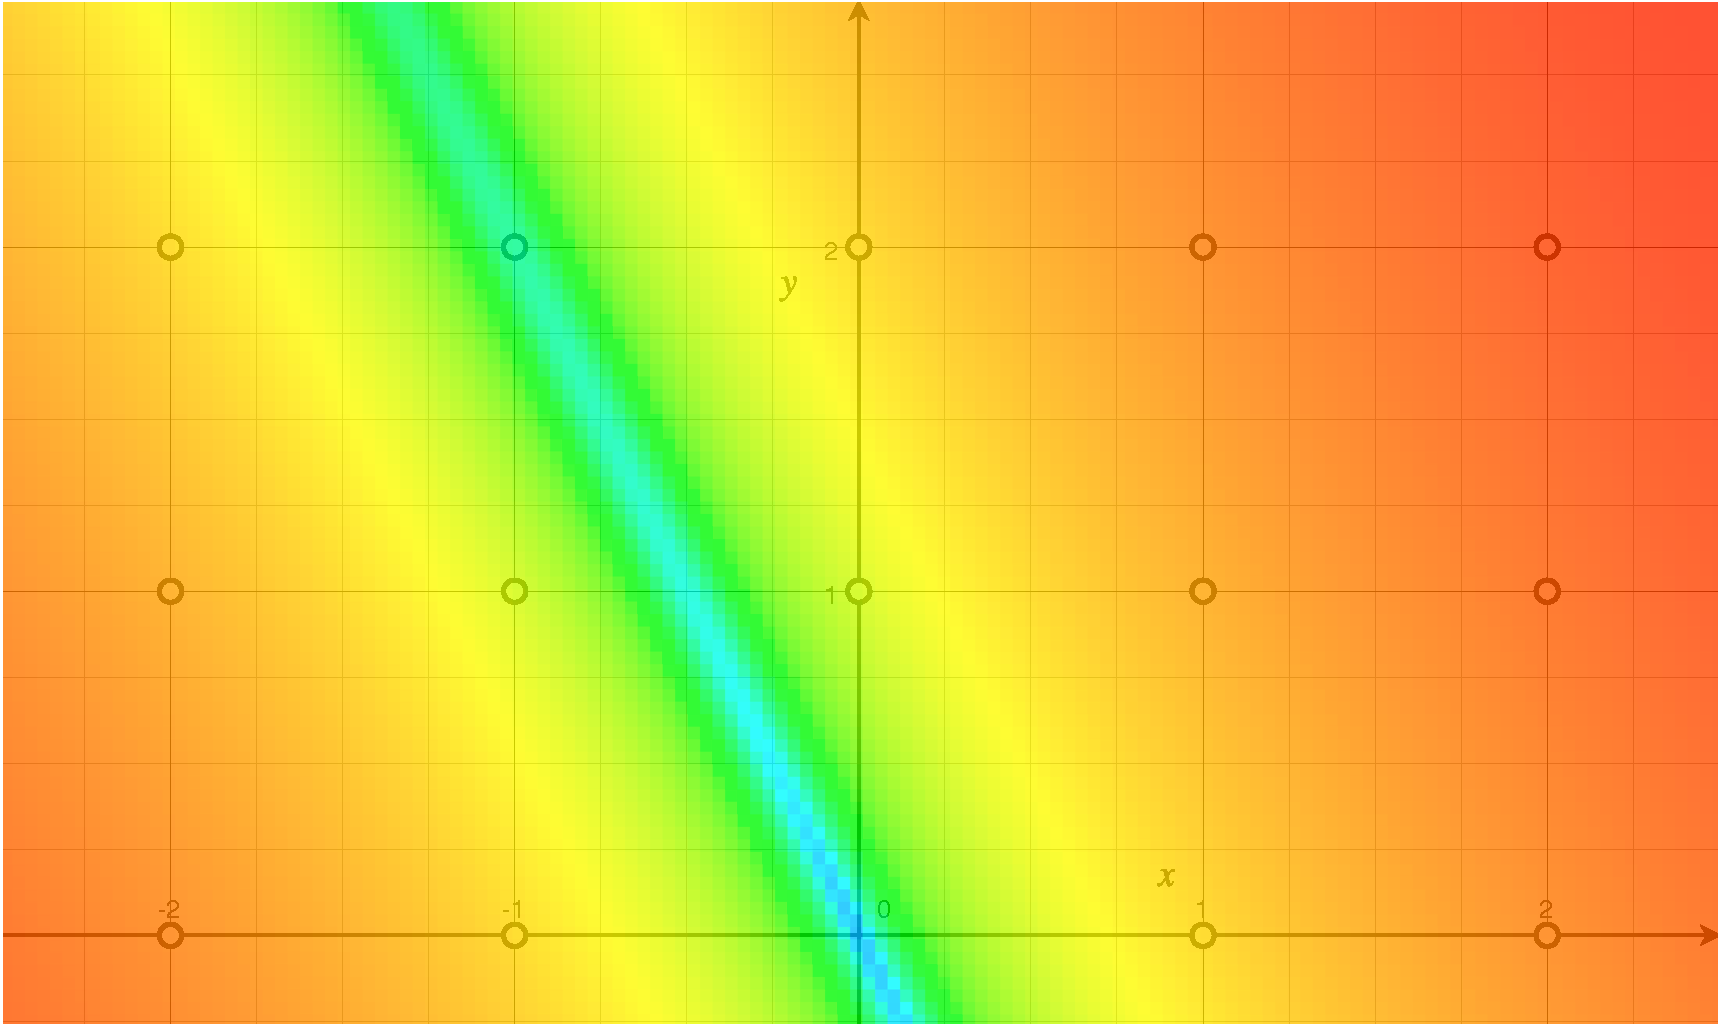
\includegraphics[width=\linewidth]{fig/lmin/80-40-2.pdf}
	\caption{$\vec{n} = \transpose{(0.894, 0.447, 0.022)}$. min: $(-1, 2)$}
\end{subfigure}
\caption{Density plot of $d(x, y)$ for different surface normal vectors $\vec{n}$}
\label{fig:lmin_d_func}
\end{figure}


\subsection{Threshold for obliqueness}
This is an attempt to define a limit, based on the normal vector $\vec{n}$ or the object surface, for when the approximation is more likely to be accurate. That is, when $\argmin d(x, y)$ is likely to be in the set $M = \{ (0, 1), (0, 1), (1, 1), (-1, 1) \}$.

The angle $\alpha$ between $\vec{n}$ and a ray from the camera with directing vector $\vec{v} = \transpose{(0, 0, -1)}$ is obtained from their dot product: $\alpha = \arccos n_z$. 

When it is $0$ the function plot becomes more radial, that is, its contour lines $d(x,y)=c$ for constant $c$ become more circular. As the angle approaches its limit $\frac{\pi}{2}$ they becomes ellipses distorted towards an angle $\beta$. When $\alpha$ is low the shape does not stretch out much to one specific direction, and the approximation is likely to be correct. This is seen in examples (a) and (b).

This direction $\beta$ in which the surface is inclined, for which $\tan \beta = \frac{n_y}{n_x}$. When it is near a multiple of $\frac{\pi}{4}$, then again it is likely that one of the points in $M$ gets the minimal value as the shape stretches in its direction, as seen on example (c). When $\beta$ it lies between those regions, and $\alpha$ is high, then a point outside of $M$ can get the minimal value, like on example (d).

This first condition is true when $|n_z| > \cos \alpha_\text{max}$, taking into account that the normal vector may point in the opposite direction. The second condition is true when $|\frac{n_x}{n_y}| < \tan \beta_{\text{max}}$ or $|\frac{n_y}{n_x}| < \tan \beta_{\text{max}}$ or $\tan \left(\frac{\pi}{4} - \beta_{\text{max}}\right) < |\frac{n_x}{n_y}| < \tan \left(\frac{\pi}{4} + \beta_{\text{max}}\right)$. Using these expressions the trigonometric functions only need to be evaluated once for the constants in an implementation.

So the threshold condition on the normal vector can be written (using $\alpha$ and $\beta$ to denote the threshold values)
\begin{equation}
|n_z| > \cos \alpha \bigvee
\left[
\left|\frac{n_x}{n_y}\right| < \tan \beta
\bigwedge \left|\frac{n_y}{n_x}\right| < \tan \beta
\bigwedge \tan \left(\tfrac{\pi}{4} - \beta\right) < \left|\frac{n_x}{n_y}\right| < \tan \left(\tfrac{\pi}{4} + \beta \right)
\right]
\end{equation}


\subsection{Density}
Evaluating $\| \vec{p'} \|$ for $(x, y) = (0, 1), (1, 0), (1, 1)$, one gets the side lengths $a, b$ of one possible parallelogram, and one if its diagonal. A diagonal splits a parallelogram into two halves into equal area. Using Heron's formula $A = \sqrt{s \, (s - a) \, (s - b) \, (s - c)}$ where $s = \frac{a+b+c}{2}$, one gets the area of the triangle with side lengths $a, b, c$, and thus the parallelogram has area $2 \, A$.

The points can be translated on the parallelogram grid such that each parallelogram contains one point and no points lie on the edges. This is not possible for a triangle grid. Counting one point per parallelogram area, the density is $\rho = \frac{1}{2 \, A}$.

Evaluating and simplifying this expression, one obtains $\rho = \frac{| n_z |}{p^2_l}$.


\begin{figure}[h]
\centering
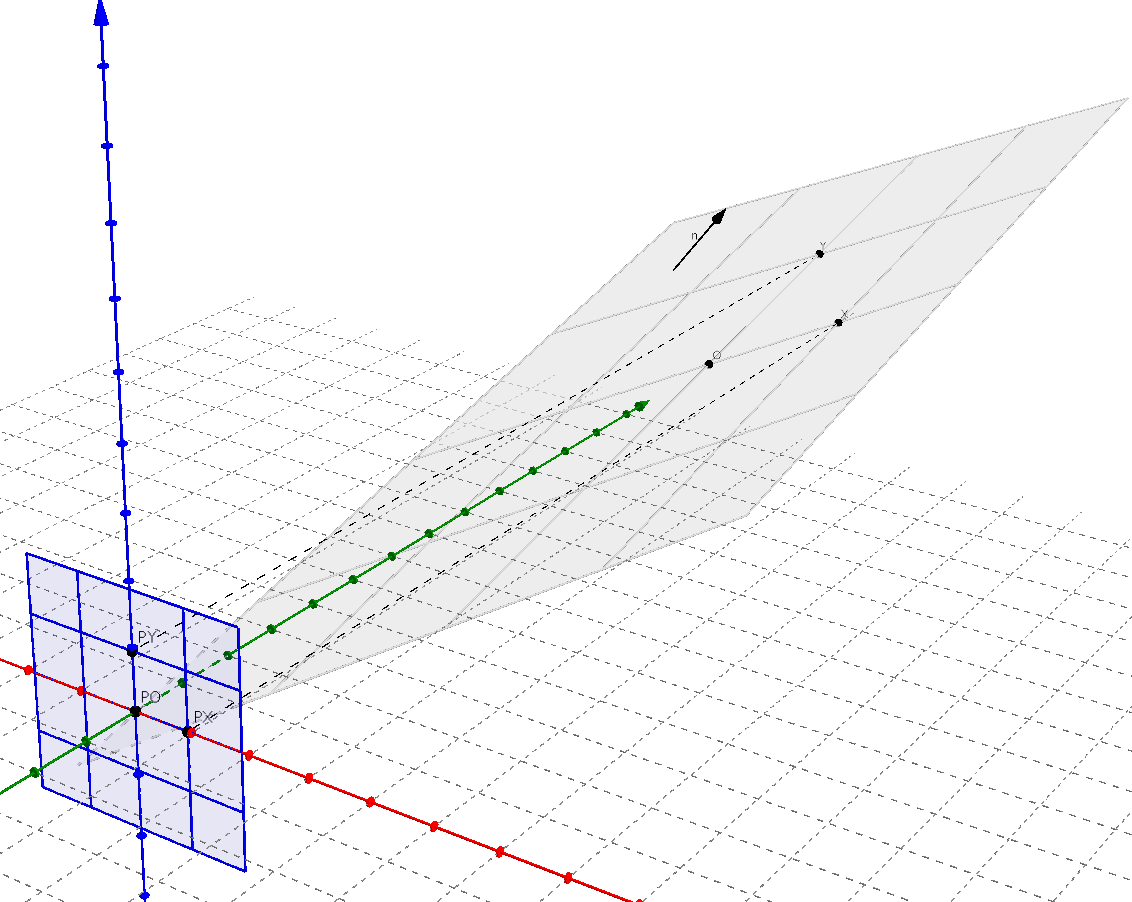
\includegraphics[width=.9\textwidth]{fig/lattice_proof.png}
\caption{Depiction of projection of image space points to parallelogram lattice on object surface}
\label{fig:lattice_proof}
\end{figure}




\section{Closest point histogram with random point dispersion on plane} \label{sec:proof_rand_disp_plane}
Point clouds $P$ and $Q$ are two perfectly aligned planes, the points $p \in P$ are randomly dispersed on $P$. $Q$ contains a large number of sample points. The probability density function for the distance of a random point $q \in Q$ to its closest neighbor in $P$ is given by
\begin{equation}
f_R(r) = 2 \pi \rho(P) \, r \, e^{-\pi \rho(P) \, r^2}
\end{equation}

\begin{proof}
Let $P$ be a bounded continuous surface in $\mathbb{R}^2$ of area $\area{P}$. For the example on the figure \ref{fig:plane_rand_d30000}, it is a square with side length $5$. Let $\{ p_i \in P \}$ be a discrete set of $n$ randomly chosen points on that surface, with an uniform probability distribution. $\rho = \frac{n}{\area{P}}$ is the surface density of this points distribution.

Let $A \subset W$ a another bounded continuous subregion of $P$, with a variable area $\area{A}$ on the order of magnitude of the distances between adjacent neighboring points $p_i$. Let $N(A) \in \mathbb{N}$ be the number of points $p_i \in P$ that lie inside $A$. In the following formulas, the area value $\area{A}$ is also denoted $A$.

For any single point $p_i \in P$, the probability that it lies in $A$, and the probability that it does not, are given by
\begin{equation} \label{eq:rand_point_in_A}
P[p_i \in A] = \frac{\area{A}}{\area{P}} = \frac{A \rho}{n}
\hspace{7mm} \text{and} \hspace{7mm}
P[p_i \notin A] = 1 - \frac{A \rho}{n}
\end{equation}

For any two $p_i$, these events are stochastically independent, and the probability that two events occur is obtained through multiplication. The probability that none of the $n$ points lie in $A$, and conversely the probability that at least one lies in $A$, are;

\begin{equation}
P[N(A) = 0] = \left(1 - \frac{A \rho}{n}\right)^n
\hspace{7mm} \text{and} \hspace{7mm}
P[N(A) \geq 1] = 1 - \left(1 - \frac{A \rho}{n}\right)^n
\end{equation}


The value $P[N(A) \geq 1]$ converges for $n \rightarrow \infty$. The information about the density of points is captured by $\rho$, so the probability be be expressed without $\area{P}$ and $n$. Setting $n' = -\frac{n}{A \, \rho}$ and using the identity $\lim_{x \rightarrow \infty} \left( 1 + \frac{1}{x} \right)^x = e$:
\begin{equation}
\begin{align}
\lim_{n \rightarrow \infty} P[N(A) \geq 1]
& = \lim_{n \rightarrow \infty} \left[ 1 - \left(1 - \frac{A \rho}{n}\right)^n \right]\\
& = 1 - \lim_{n \rightarrow \infty} \left(1 - \frac{A \rho}{n}\right)^n \\
& = 1 - \lim_{n' \rightarrow \infty} \left(1 + \frac{1}{n'}\right)^{-A \rho \, n'}\\
& = 1 - \left[ \lim_{n' \rightarrow \infty} \left(1 + \frac{1}{n'}\right)^{n'} \right]^{-A \rho}\\
& = 1 - e^{-A \rho}
\end{align}
\label{eq:leastone_point_prob}
\end{equation}
For the final expression $A \in \mathbb{R}$ denotes only the area, as no further information on the region's shape is needed. 

The goal what to find the underlying curve of the histogram in \ref{fig:plane_rand_d30000}. In order to obtain a smooth function, the histogram taken with a sparse set of points $q \in Q$ is replaced by a probability density function of the closest point distance from any $q \in Q$ to its nearest neighbor $p_i \in P$. The surfaces $P$ and $Q$ are the same.

Let $q \in P$ be any point lying on the plane $P$. (Not necessarily one of the discrete set of points $p_i$.) Let $D_{q,r} \in P$ be the disk centered at $q$ with radius $r$. Its area is $\area{D_{r}} = \pi r^2$. By definition, for any point $p \in D_{q,r}$, $\| p - q \| \leq r$. Starting from $r = 0$, the radius of the disk is increased until $N(D_{q,r}) = 1$. $r = r_{\text{closest}}$ is then the closest point distance to $q$.

One has $r \geq r_{\text{closest}}$ if and only if $N(D_{q,r}) \geq 1$: ($\Rightarrow$) As $r$ gets larger, the disk can be made to contain additional points, but no points get removed. It contains one point when $r = r_{\text{closest}}$ (or possibly multiple equidistant points). ($\Leftarrow$) For the disk to contain one point, it must at least have a radius large enough to contain the closest point to $q$.

Let $R : q \mapsto r_{\text{closest}}$ be the random variable expressing the distance from any $q \in P$ to its closest neighbor. Now $P[R \leq r] = P[N(D_{r}) \geq 1]$. The probability density function $f_R(r)$ is obtained by differentiating:
\begin{equation}
\begin{align}
f_R(r)
& = \frac{\diffd}{\diffd r} P[R \leq r] = \frac{\diffd}{\diffd r} P[N(D_{r}) \geq 1]\\
& = \frac{\diffd}{\diffd r} \left( 1 - A \rho \, e^{-A \rho} \right)\\
& = - \frac{\diffd}{\diffd r} e^{-A \rho}\\
& = - \frac{\diffd}{\diffd r} e^{-\pi \rho \, r^2}\\
& = 2 \pi \rho \, r \, e^{-\pi \rho \, r^2}
\end{align}
\end{equation}
\end{proof}




\section{Variance of density with random point dispersion}  \label{sec:proof_var_rand_pt_disp}
The density of points dispersed on a plane is defined as $\rho = \frac{N(A)}{A}$, where $N(A)$ is the number of points in an area $A$.

The probability $P[N(A) = m]$ is given by
\begin{equation} \label{eq:rand_m_points_in_A}
P[N(A) = m] = \binom{n}{m} \, \left( \frac{A \rho}{n} \right)^m \, \left( 1 - \frac{A \rho}{n} \right)^{n-m}
\end{equation}

\begin{proof}
Each of the $n$ points $p_i \in P$ may lie inside or outside of $A$. The probabilities of these events are given in equation \ref{eq:rand_point_in_A}, and they are stochastically independent. For there to be exactly $m$ points inside $A$, the event $p_i \in A$ must occur $m$ times, and the event $p_i \notin A$ must occur $n - m$ times.
By commutativity of the product, the probability for each one of those sequences of events to occur is always
\begin{equation}
\left( \frac{A \rho}{n} \right)^m \, \left( 1 - \frac{A \rho}{n} \right)^{n-m}
\end{equation}
Since there are $\binom{n}{m}$ such sequences, and they are mutually exclusive, the probability for any one of them to occur is the expression given in \ref{eq:rand_m_points_in_A}.
\end{proof}

It is not a single spike at the expected value $\bar{N}(A) = A \, \rho$, and the most likely outcome can be different from the expected value. Figure \ref{fig:plane_rand_n} shows $P[N(A) = m]$ and $\bar{N}(A)$, interpolated to use real values for $N(A)$.

\begin{figure}[h]
\centering
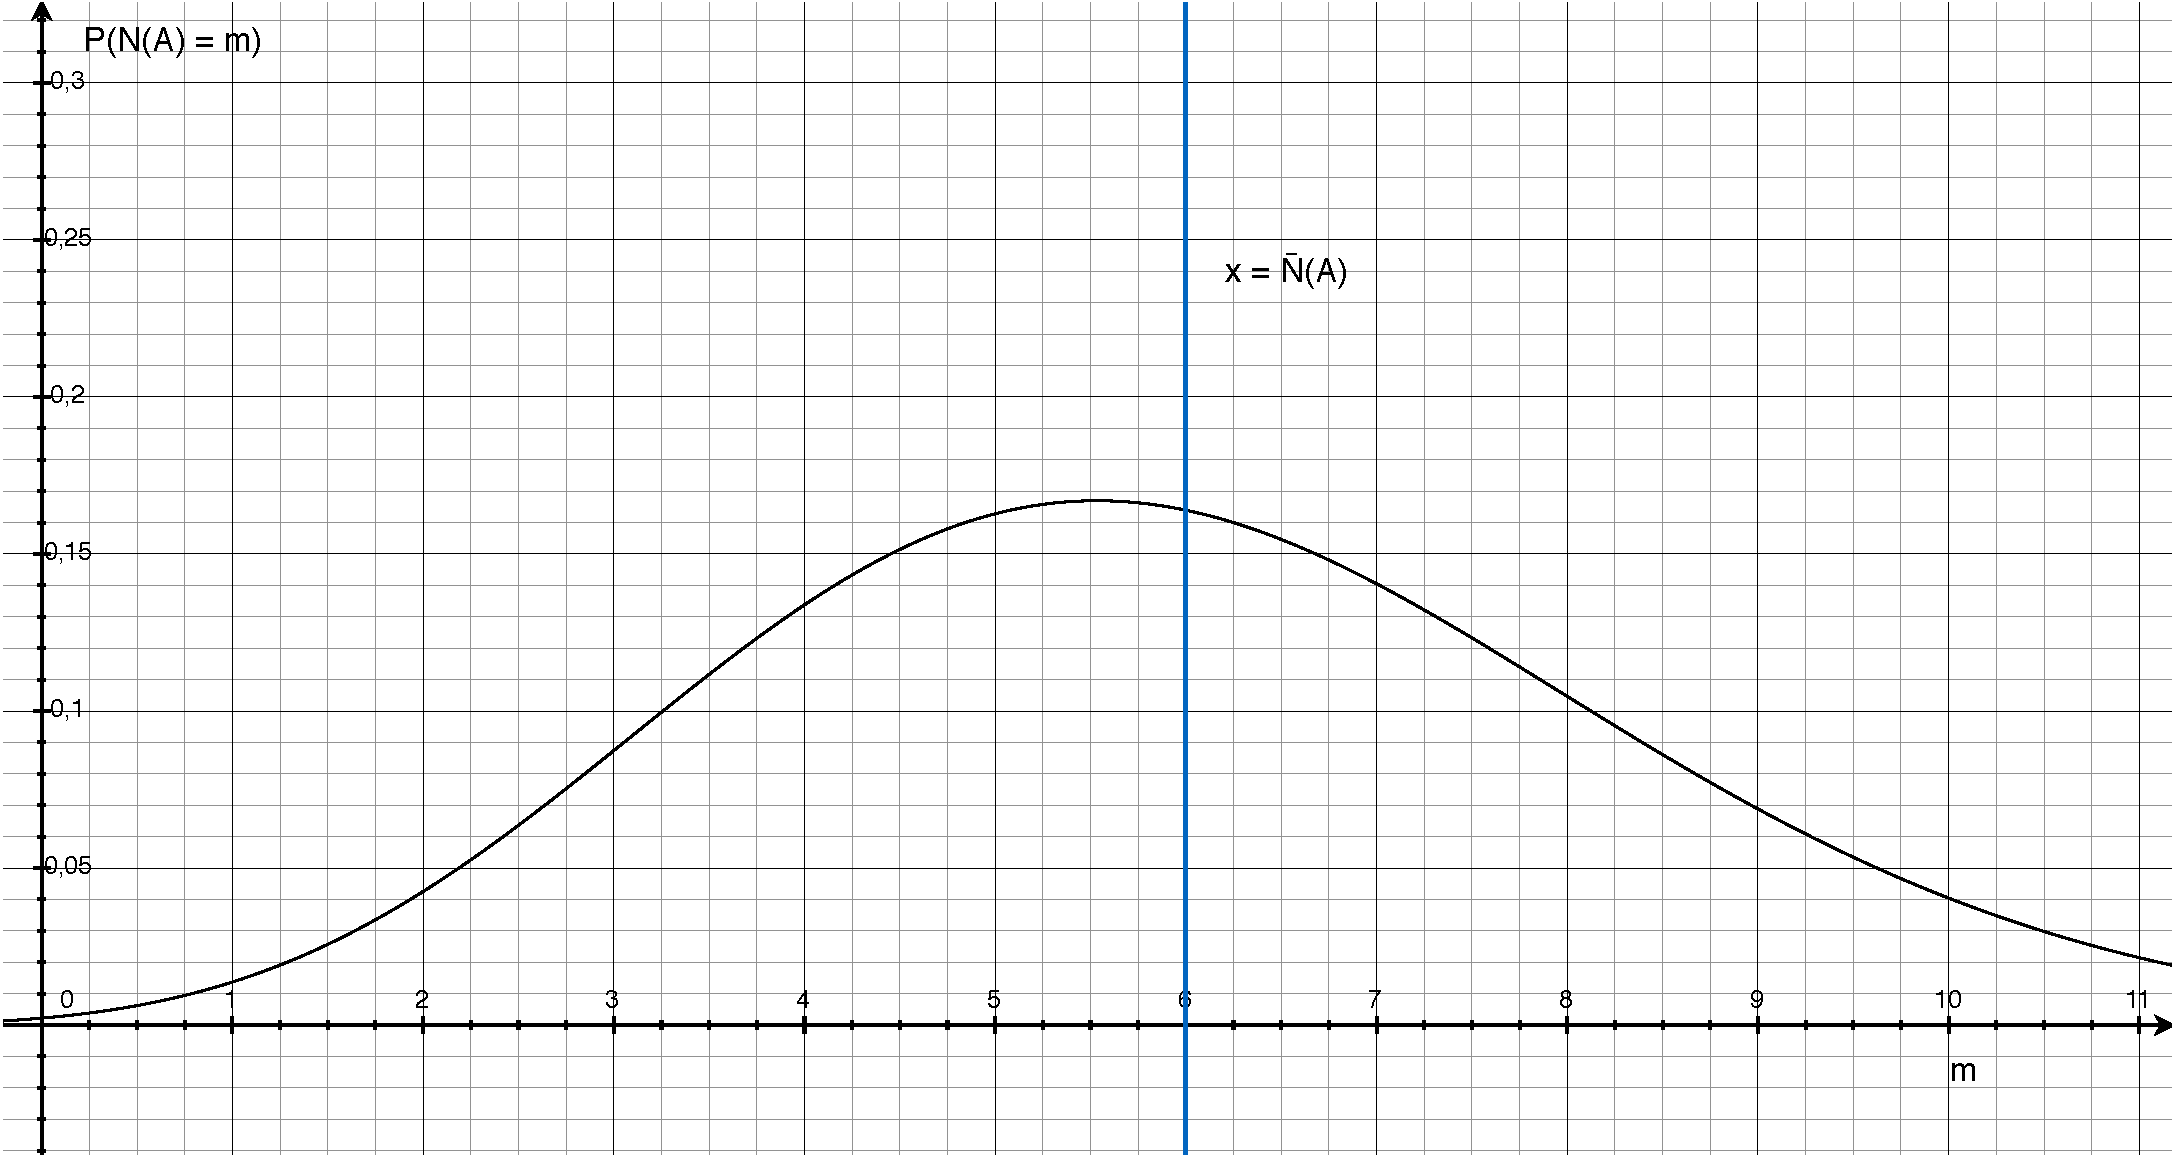
\includegraphics[width=.6\textwidth]{fig/plane_rand_n.pdf}
\caption{$P[N(A) = m]$ for randomly dispersed points on a plane, interpolated to real values}
\label{fig:plane_rand_n}
\end{figure}


\section{Closest point histogram with square grid point dispersion on plane} \label{sec:proof_sqgrid_disp_plane}
Under the assumption of two perfectly aligned planar surfaces $P$ and $Q$, where points on $P$ are arranged on a square grid with surface density $\rho(P)$, the probability density function $f_R$ is
\begin{equation}
f_R(r) = \frac{1}{2 l} \times \begin{cases}
	\frac{\pi}{4} \, r & 0 \leq r \leq \frac{l}{2} \\
	\left( \frac{\pi}{4} - \arctan{\sqrt{\left( \frac{2r}{l} \right)^2 - 1}} \right) r & \frac{l}{2} < r < \frac{l}{2} \sqrt{2}
\end{cases}
\end{equation}
with $l = \frac{1}{\sqrt{\rho(P)}}$.

\begin{proof}
The points are arranged on a square grid, with side length $l$. For the purpose of the following explanation, let $l = 2$.

Figure \ref{fig:sq_grid} shows four points $p_1, p_2, p_3, p_4 \in P$ with two-dimensional coordinates, and a point $q$ that lies on the same plane as those four points. The background color indicates for each position the distance to the closest point of $P$. It remains constant on each of the white contour lines. $d(q, P)$ is maximal when $q$ is in the center of one of the squares, as it does on the figure. So $d_{\text{max}} = \sqrt{2}$.

The histogram corresponds to the probability distribution of $d(q, P)$. The entire plane can be tiled with the triangle $\Delta$ which is drawn in the figure, with the probability distribution being the same in each of these tiles, as the $\Delta$ would only get flipped along one of its sides. So it is sufficient to only look at the field within $\Delta$. Its side lengths are $1, 1, \sqrt{2}$, and its angle at the point $p_1 = (0, 0)$ is $\frac{\pi}{8}$. For each point inside $\Delta$, $p_1$ is its closest point in $P$.

Each value for $d \in [0, d_{\text{max}}]$ occurs in $\Delta$, exactly at the points that lie on the arc formed by the intersection of $\Delta$ and the circle $C_d$ of radius $d$. Let $a(d)$ be the length of this arc in function of $d$. On the figure, $k$ is the intersection point of $\overline{p_1 q}$ with $C_1$. When $d \leq 1$, the arc ranges from the abscissa axis to the diagonal, which is one eight of the circle, and so $a_1(d) = \frac{\pi}{4} \, d$.

When $1 < d < d_{\text{max}}$, it is additionally cut off by the line $x = 1$. By solving $(x, y) \in C_d \wedge x = 1$, its intersection point with that line is $(1, \sqrt{d^2 - 1})$. Instead of starting from the abscissa, the remaining arc now starts from $\varphi = \arctan{\sqrt{d^2 - 1}}$, and so $a_2(d) = (\frac{\pi}{4} - \varphi) \, d$. The function $a$ is
\begin{equation}
a(d) = \begin{cases}
	\frac{\pi}{4} \, d & 0 \leq d \leq 1 \\
	\left( \frac{\pi}{4} - \arctan{\sqrt{d^2 - 1}} \right) \, d & 1 < d < \sqrt{2}
\end{cases}
\end{equation}
under the assumption that $l = 2$.

Removing this assumption, $l$ is now determined as a function of the surface points density $\rho$. The density is constant throughout the surface, so $\rho$ expresses the number of points that lie inside any region of $P$, divided by the area of that region. The area of a square region formed by four points is $l^2$. After a small translation of the point in any direction so that they don't lie on the region's borders, there is $1$ point in each $l^2$ region. So $\rho = \frac{1}{l^2}$ and $l = \frac{1}{\sqrt{\rho}}$. In this general case, the function $a$ becomes
\begin{equation}
a(d) = \frac{l}{2} \times \begin{cases}
	\frac{\pi}{4} \, d & 0 \leq d \leq \frac{l}{2} \\
	\left( \frac{\pi}{4} - \arctan{\sqrt{\left( \frac{2d}{l} \right)^2 - 1}} \right) \, d & \frac{l}{2} < d < \frac{l}{2} \sqrt{2}
\end{cases}
\end{equation}

Since the arcs completely completely cover $\Delta$ and none of them overlap, $\int a(d) \, \diffd d = \area{\Delta} = l^2$. Normalizing the integral to $1$, the probability density function $f_R$ becomes
\begin{equation}
f_R(d) = \frac{a(d)}{l^2}
\end{equation}

\begin{figure}[h]
\centering
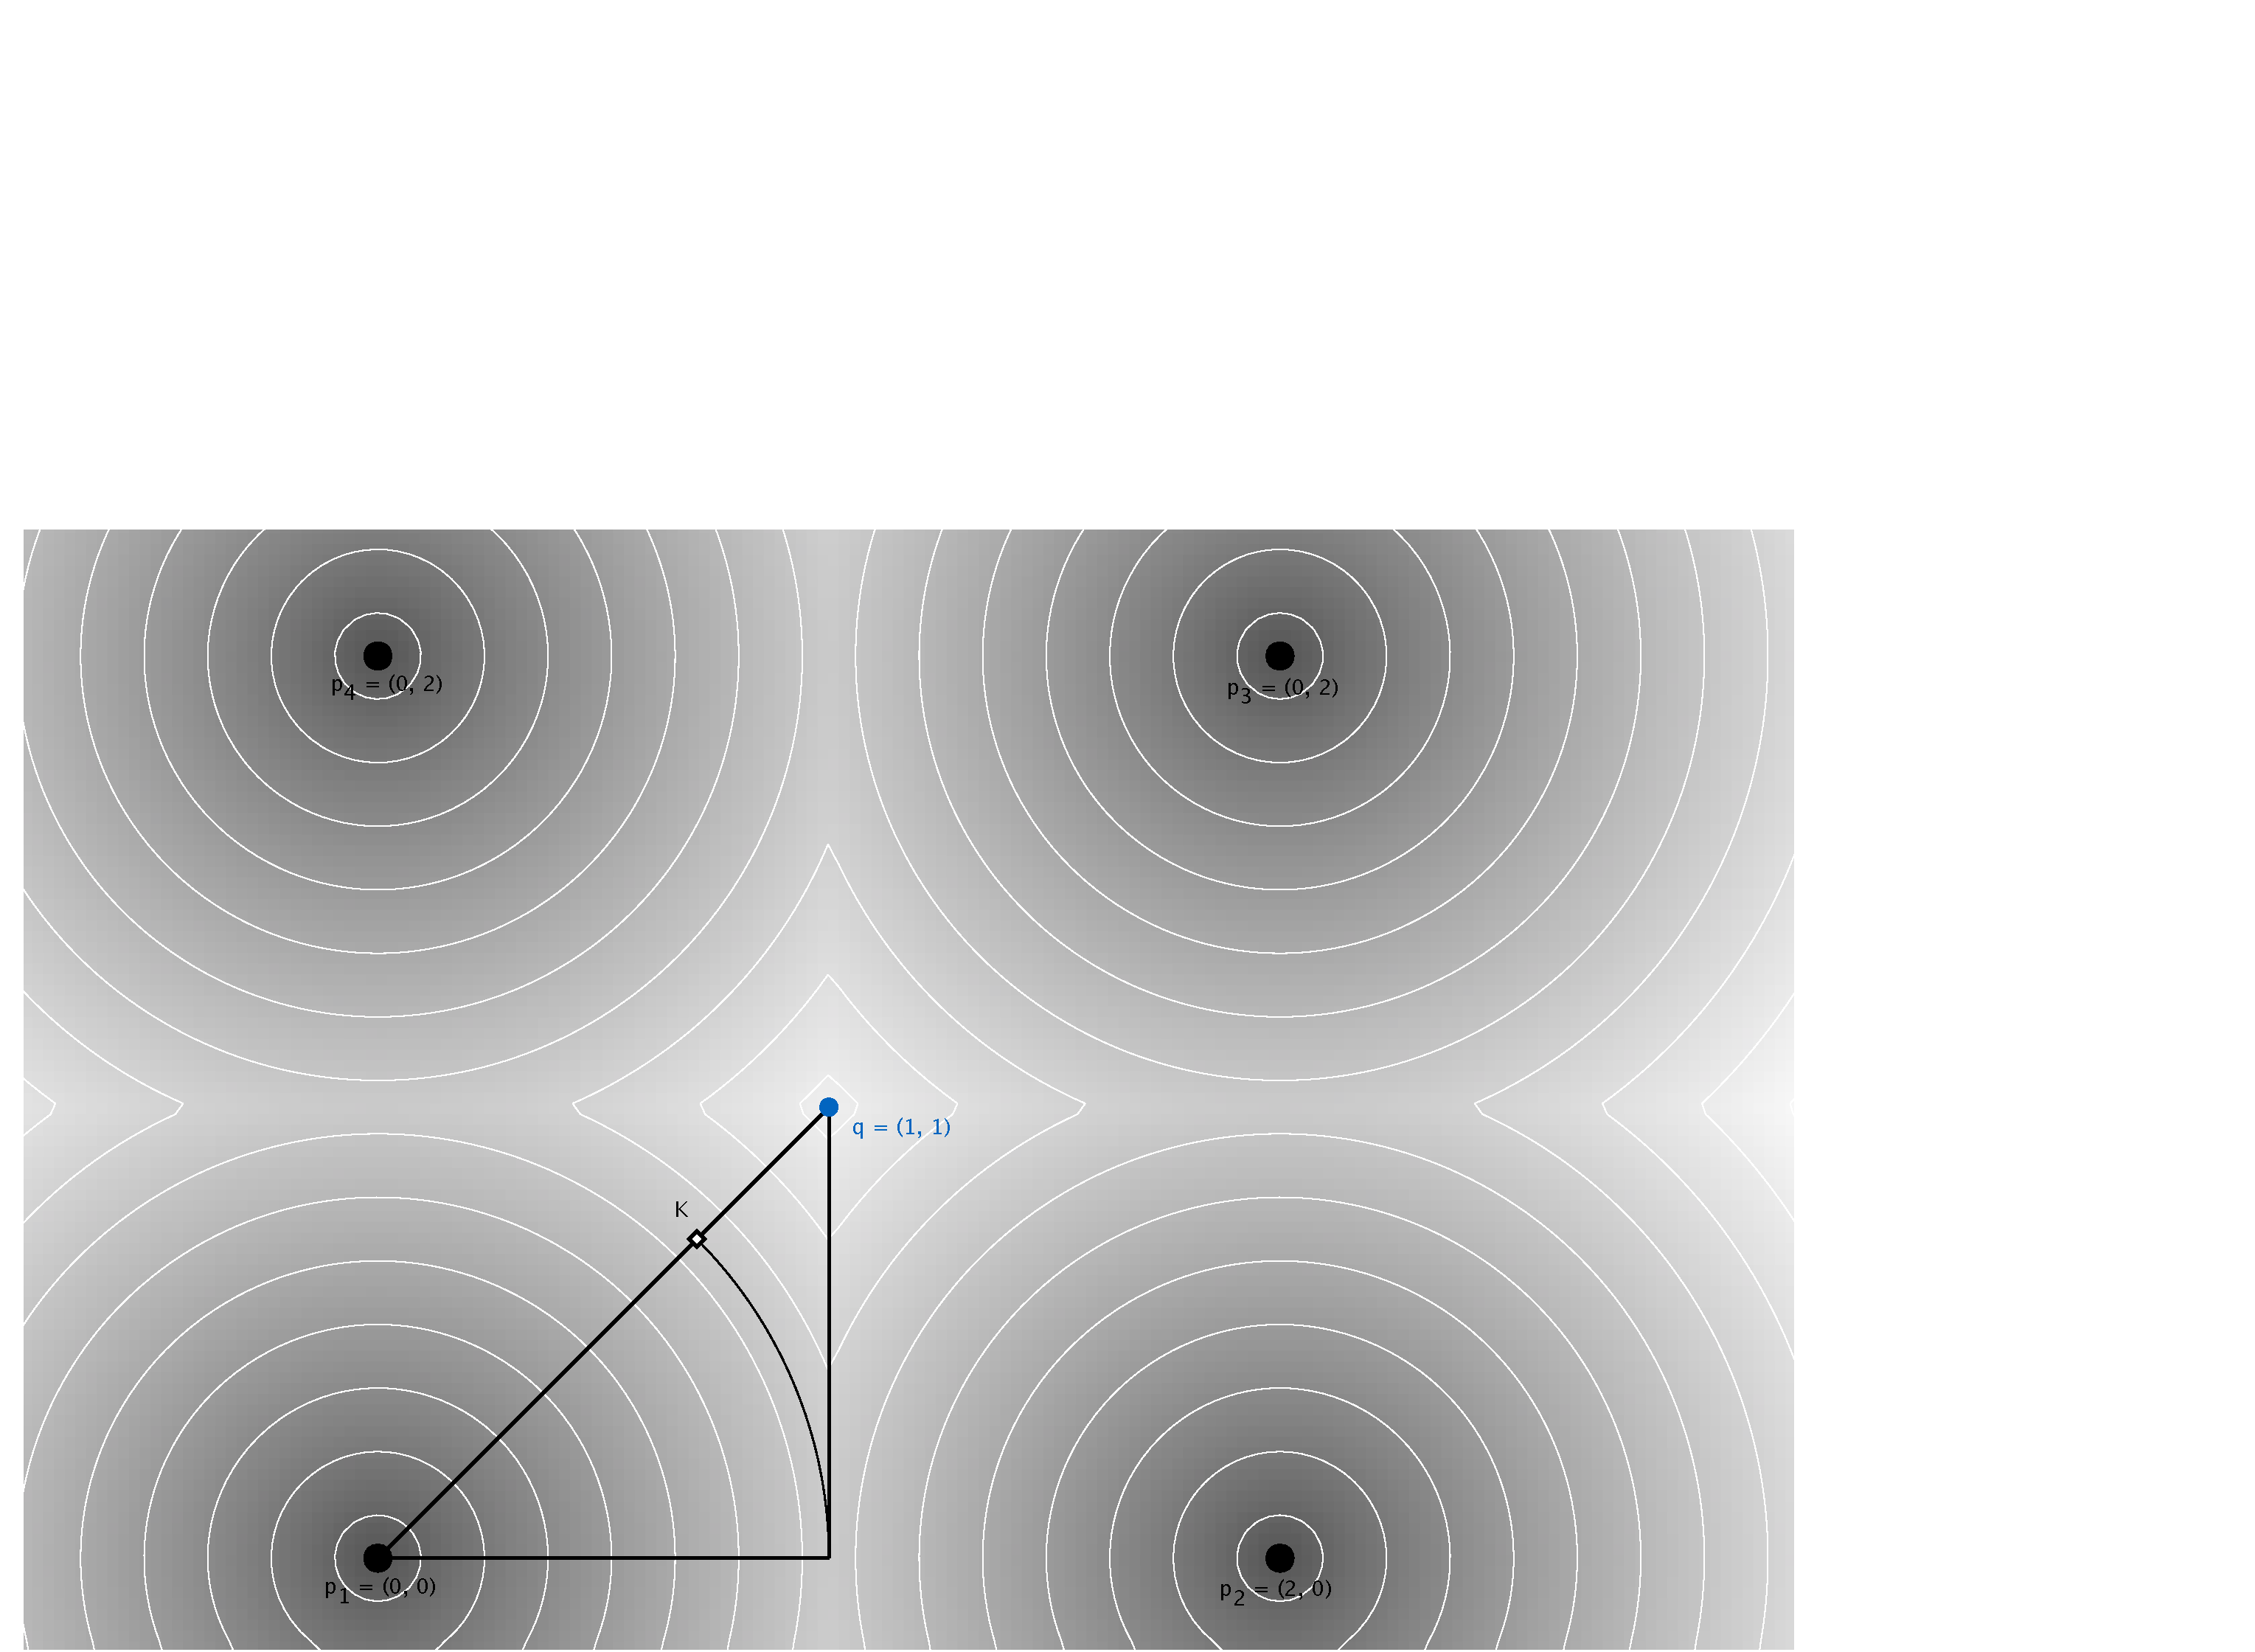
\includegraphics[width=.8\textwidth]{fig/sq_grid.pdf}
\caption{Closest points distance field with square grid distribution of $P$, $l = 2$}
\label{fig:sq_grid}
\end{figure}

\end{proof}
